\PassOptionsToPackage{unicode=true}{hyperref} % options for packages loaded elsewhere
\PassOptionsToPackage{hyphens}{url}
%
\documentclass[]{article}
\usepackage{lmodern}
\usepackage{amssymb,amsmath}
\usepackage{ifxetex,ifluatex}
\usepackage{fixltx2e} % provides \textsubscript
\ifnum 0\ifxetex 1\fi\ifluatex 1\fi=0 % if pdftex
  \usepackage[T1]{fontenc}
  \usepackage[utf8]{inputenc}
  \usepackage{textcomp} % provides euro and other symbols
\else % if luatex or xelatex
  \usepackage{unicode-math}
  \defaultfontfeatures{Ligatures=TeX,Scale=MatchLowercase}
\fi
% use upquote if available, for straight quotes in verbatim environments
\IfFileExists{upquote.sty}{\usepackage{upquote}}{}
% use microtype if available
\IfFileExists{microtype.sty}{%
\usepackage[]{microtype}
\UseMicrotypeSet[protrusion]{basicmath} % disable protrusion for tt fonts
}{}
\IfFileExists{parskip.sty}{%
\usepackage{parskip}
}{% else
\setlength{\parindent}{0pt}
\setlength{\parskip}{6pt plus 2pt minus 1pt}
}
\usepackage{hyperref}
\hypersetup{
            pdftitle={ComSci Project - MyTime},
            pdfauthor={Max Stupple},
            pdfborder={0 0 0},
            breaklinks=true}
\urlstyle{same}  % don't use monospace font for urls
\usepackage{color}
\usepackage{fancyvrb}
\newcommand{\VerbBar}{|}
\newcommand{\VERB}{\Verb[commandchars=\\\{\}]}
\DefineVerbatimEnvironment{Highlighting}{Verbatim}{commandchars=\\\{\}}
% Add ',fontsize=\small' for more characters per line
\newenvironment{Shaded}{}{}
\newcommand{\AlertTok}[1]{\textcolor[rgb]{1.00,0.00,0.00}{\textbf{#1}}}
\newcommand{\AnnotationTok}[1]{\textcolor[rgb]{0.38,0.63,0.69}{\textbf{\textit{#1}}}}
\newcommand{\AttributeTok}[1]{\textcolor[rgb]{0.49,0.56,0.16}{#1}}
\newcommand{\BaseNTok}[1]{\textcolor[rgb]{0.25,0.63,0.44}{#1}}
\newcommand{\BuiltInTok}[1]{#1}
\newcommand{\CharTok}[1]{\textcolor[rgb]{0.25,0.44,0.63}{#1}}
\newcommand{\CommentTok}[1]{\textcolor[rgb]{0.38,0.63,0.69}{\textit{#1}}}
\newcommand{\CommentVarTok}[1]{\textcolor[rgb]{0.38,0.63,0.69}{\textbf{\textit{#1}}}}
\newcommand{\ConstantTok}[1]{\textcolor[rgb]{0.53,0.00,0.00}{#1}}
\newcommand{\ControlFlowTok}[1]{\textcolor[rgb]{0.00,0.44,0.13}{\textbf{#1}}}
\newcommand{\DataTypeTok}[1]{\textcolor[rgb]{0.56,0.13,0.00}{#1}}
\newcommand{\DecValTok}[1]{\textcolor[rgb]{0.25,0.63,0.44}{#1}}
\newcommand{\DocumentationTok}[1]{\textcolor[rgb]{0.73,0.13,0.13}{\textit{#1}}}
\newcommand{\ErrorTok}[1]{\textcolor[rgb]{1.00,0.00,0.00}{\textbf{#1}}}
\newcommand{\ExtensionTok}[1]{#1}
\newcommand{\FloatTok}[1]{\textcolor[rgb]{0.25,0.63,0.44}{#1}}
\newcommand{\FunctionTok}[1]{\textcolor[rgb]{0.02,0.16,0.49}{#1}}
\newcommand{\ImportTok}[1]{#1}
\newcommand{\InformationTok}[1]{\textcolor[rgb]{0.38,0.63,0.69}{\textbf{\textit{#1}}}}
\newcommand{\KeywordTok}[1]{\textcolor[rgb]{0.00,0.44,0.13}{\textbf{#1}}}
\newcommand{\NormalTok}[1]{#1}
\newcommand{\OperatorTok}[1]{\textcolor[rgb]{0.40,0.40,0.40}{#1}}
\newcommand{\OtherTok}[1]{\textcolor[rgb]{0.00,0.44,0.13}{#1}}
\newcommand{\PreprocessorTok}[1]{\textcolor[rgb]{0.74,0.48,0.00}{#1}}
\newcommand{\RegionMarkerTok}[1]{#1}
\newcommand{\SpecialCharTok}[1]{\textcolor[rgb]{0.25,0.44,0.63}{#1}}
\newcommand{\SpecialStringTok}[1]{\textcolor[rgb]{0.73,0.40,0.53}{#1}}
\newcommand{\StringTok}[1]{\textcolor[rgb]{0.25,0.44,0.63}{#1}}
\newcommand{\VariableTok}[1]{\textcolor[rgb]{0.10,0.09,0.49}{#1}}
\newcommand{\VerbatimStringTok}[1]{\textcolor[rgb]{0.25,0.44,0.63}{#1}}
\newcommand{\WarningTok}[1]{\textcolor[rgb]{0.38,0.63,0.69}{\textbf{\textit{#1}}}}
\usepackage{graphicx,grffile}
\makeatletter
\def\maxwidth{\ifdim\Gin@nat@width>\linewidth\linewidth\else\Gin@nat@width\fi}
\def\maxheight{\ifdim\Gin@nat@height>\textheight\textheight\else\Gin@nat@height\fi}
\makeatother
% Scale images if necessary, so that they will not overflow the page
% margins by default, and it is still possible to overwrite the defaults
% using explicit options in \includegraphics[width, height, ...]{}
\setkeys{Gin}{width=\maxwidth,height=\maxheight,keepaspectratio}
\setlength{\emergencystretch}{3em}  % prevent overfull lines
\providecommand{\tightlist}{%
  \setlength{\itemsep}{0pt}\setlength{\parskip}{0pt}}
\setcounter{secnumdepth}{0}
% Redefines (sub)paragraphs to behave more like sections
\ifx\paragraph\undefined\else
\let\oldparagraph\paragraph
\renewcommand{\paragraph}[1]{\oldparagraph{#1}\mbox{}}
\fi
\ifx\subparagraph\undefined\else
\let\oldsubparagraph\subparagraph
\renewcommand{\subparagraph}[1]{\oldsubparagraph{#1}\mbox{}}
\fi

% set default figure placement to htbp
\makeatletter
\def\fps@figure{htbp}
\makeatother


\title{ComSci Project - MyTime}
\author{Max Stupple}
\date{}

\begin{document}
\maketitle

\hypertarget{analysis}{%
\section{Analysis}\label{analysis}}

\hypertarget{overview-of-the-problem}{%
\subsubsection{Overview of the problem}\label{overview-of-the-problem}}

Many students struggle to manage their time. The workload of A-levels
alone is enough to make it difficult to balance between small pieces
that are due in soon, and longer project that need a little bit of work
here and there, let alone extra-curricular activities and sports that
take up more time after school and on weekends. One solution is to
manually plan how you will use all your free time, but this has two
drawbacks:

\begin{itemize}
\item
  Many people struggle to estimate how long a task will take them and
  hence struggle to allocate a reasonable amount of time to each task
\item
  This process takes time, a resource which has already been established
  to be finite and valuable
\end{itemize}

My stakeholder (henceforth referred to as SH) is a Year 12 Sixth Form
student studying Maths, Further Maths, Physics and Chemistry. He
struggles to fit in all his work around his various extra-curricular
activities, so he needs an app that will not only help him keep track of
what he needs to do, but timetable when to do each task and prioritise
those which are most urgent. SH represents the needs of my target user
group.

\hypertarget{limitations-of-current-system}{%
\subsubsection{Limitations of current
system}\label{limitations-of-current-system}}

To organise his tasks, SH currently uses the Apple Reminders app on his
iPhone. However, he finds this lacking for a number of reasons. Although
the app helps him keep track of the tasks he needs complete and when
they are due, it does not help him prioritise these tasks or inform him
of the relationship between the amount of time he needs to do those
tasks and the amount of time he has before they are due. He also doesn't
find the app very engaging, as he lacks a sense of accomplishment after
completing a task and ticking it off his list. Furthermore, the app only
provides the ability to sync between Apple devices, which he finds
limiting as he cannot access his tasks on his Windows computer. SH also
finds the light theme of the app abhorrent, and desires a solution with
a darker, more attractive colour scheme.

\hypertarget{initial-ideas}{%
\subsubsection{Initial ideas}\label{initial-ideas}}

This initial feature list will help me research existing software which
may partially solve the problem. It will also give an idea of how
complex the final solution will be.

To satisfy the needs of SH, I anticipate a solution will need to fulfil
the following functions:

\begin{itemize}
\item
  Keep a list of the users tasks which contain a description of the
  task, a due date and time estimate
\item
  Schedule tasks in user's free time according to a calendar and
  school/work schedule
\item
  Record and track the actual time taken to complete a task, including
  breaks
\item
  Provide feedback on the accuracy of the user's time estimates and
  productivity levels
\item
  Adapt to the user's preference in terms of length of work sessions
\item
  Display these tasks to the user is an organised manner using a
  Graphical User Interface
\end{itemize}

The program will be created as a web app using the Django web framework.
The reason for creating it as a web app is so that it is available as
widely as possible, as it will be possible to access it on any device
with a modern web browser. Django will allow me to deploy my solution in
a modern and efficient way, so that I can focus on the underlying data
structures, while Django mostly handles the interface. The data
structures will also be implemented using Python in an object-oriented
way, which I think is sensible and are tools I'm familiar with working
with.

\hypertarget{user-group}{%
\subsubsection{User group}\label{user-group}}

My target users are students, in particular Sixth Form and University.
As the program is targeted at individuals who struggle to manage their
time and avoid procrastination, the program will need to be engaging and
provide incentives for the user to complete tasks early rather than
delaying them. Thus the user will avoid situations in which they find
themselves with insufficient time to complete all their tasks before
they are due.

The UI must also be simple and intuitive to use: there's no point in
using an app to organise your time if you waste more time trying to get
the app to work than doing the work you need to do.

\hypertarget{computational-methods}{%
\subsubsection{Computational methods}\label{computational-methods}}

This problem lends itself to a computational solution in particular due
to the need for automation and interactivity to ensure engagement. One
potential non-computational solution could be a physical calendar or
to-do list, however this would not be able to provide the features
required by my client. Such a solution could not automatically allocate
time for the user to complete their tasks in, and could not remind the
user of their tasks - it would require the user to check and plan the
time for themselves.

\hypertarget{abstraction}{%
\paragraph{Abstraction}\label{abstraction}}

Data will be stored with an object-oriented approach. Tasks, events,
routine events, and allocated time slots will all be objects with
appropriate relationships so that the data can be viewed from a number
of perspectives.

\hypertarget{reusability}{%
\paragraph{Reusability}\label{reusability}}

There are a number of functions which my program will need to perform
where it wouldn't make sense to write them myself from scratch, so I
will use libraries that have already solved the problem. I will need to
be able to get the current date and time, to associate with each task,
and a SQL database to store my data in.

\hypertarget{visualisation}{%
\paragraph{Visualisation}\label{visualisation}}

My program will need to be able to present data to the user in a way
that is visually appealing and easy to understand. For example, data
about the number of tasks completed can be presented on a histogram.

\hypertarget{concurrency}{%
\paragraph{Concurrency}\label{concurrency}}

The program will need to be able to perform certain tasks in the
background without interrupting the user, for example allocating time
slots to tasks and analysing data to create graphs and provide feedback
to the user.

\hypertarget{data-mining}{%
\paragraph{Data Mining}\label{data-mining}}

Albeit on a small scale, my program will use the concept of data mining
to analyse trends in the user's completion of tasks, such as how much
time they spend and how accurate their time estimates are, in order to
give feedback and help the user improve their efficiency.

\hypertarget{logic}{%
\paragraph{Logic}\label{logic}}

The program will need to be able to intelligently allocate time slots to
tasks based on the user's schedule and the time needed to complete the
task. It will also need to be able to adapt the user's habits and
preferences regarding their work schedule.

\hypertarget{research}{%
\subsubsection{Research}\label{research}}

I identified a number of candidates for solutions to SH's problem. The
candidate programs are:

\begin{itemize}
\item
  Forest
\item
  Evernote
\item
  Todoist
\item
  Remember the Milk
\item
  Ike
\item
  Google Keep
\item
  Trello
\end{itemize}

\begin{figure}
\hypertarget{fig:forest1}{%
\centering
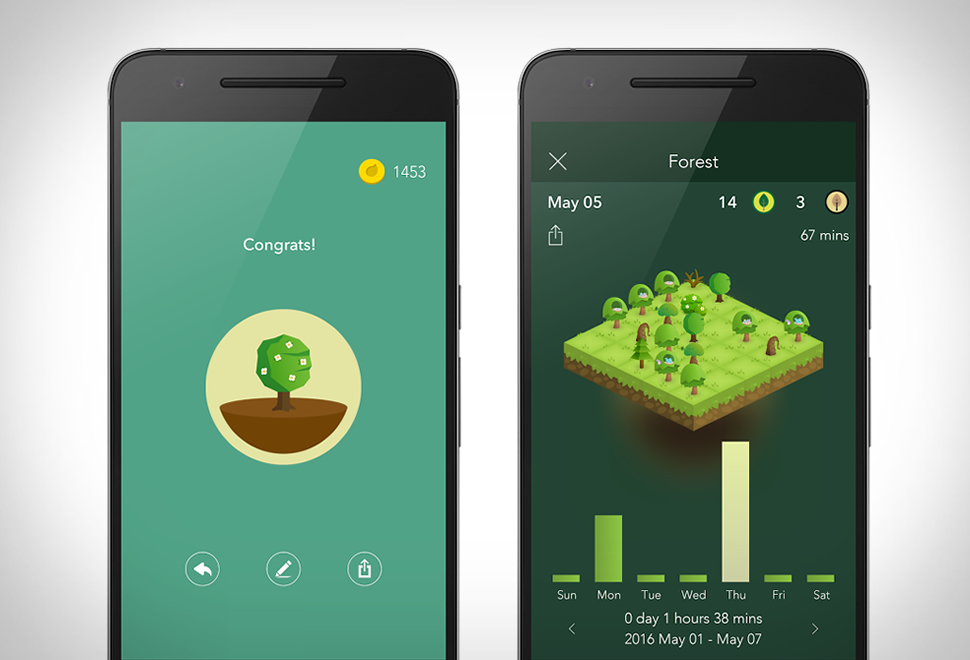
\includegraphics{./tex2pdf.-ae8b3c0afe160db8/a3e4542973b17b9d6b65c99952603f0d741f1d42.jpg}
\caption{Forest{}}\label{fig:forest1}
}
\end{figure}

Forest is the only candidate dedicated to helping the user focus on
their tasks and get stuff done as quickly as possible by avoiding
distractions. It's primary feature is an animated forest which grows as
you work, but dies if you leave the app. This encourages the user to
avoid 'quickly' having a look at Facebook, sending a text or otherwise
breaking their workflow. Forest shows you how much time you spent each
day growing your forest, so you can see which days you were most
productive on. The primary drawback of Forest is that it lacks any means
of tracking tasks from within the app. In my view this is significantly
problematic as the app which is going to help you focus the most is one
which never needs you to leave while working. Integrated task management
is an absolute must for my solution.

\begin{figure}
\hypertarget{fig:evernote1}{%
\centering
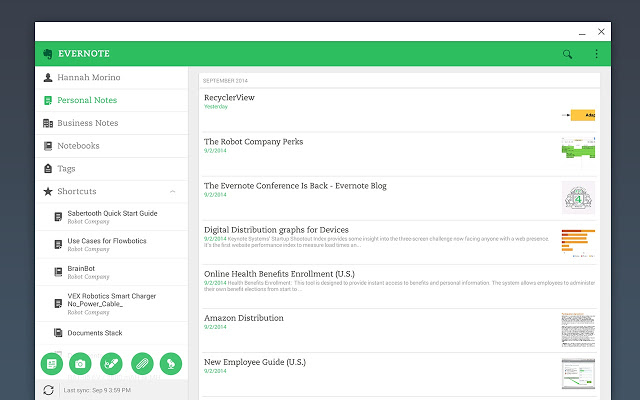
\includegraphics{./tex2pdf.-ae8b3c0afe160db8/5fe1d1ca864b78d8b632b8b2190688f288849d8a.jpg}
\caption{Evernote{}}\label{fig:evernote1}
}
\end{figure}

Evernote is primarily focused on note-taking, organisation and
task-management. The power of it's note-taking is remarkable, and can
include voice memos, handwritten notes and embedded web pages. However,
most of these features are superfluous for my product, and would
needlessly add complexity.

\begin{figure}
\hypertarget{fig:todoist1}{%
\centering
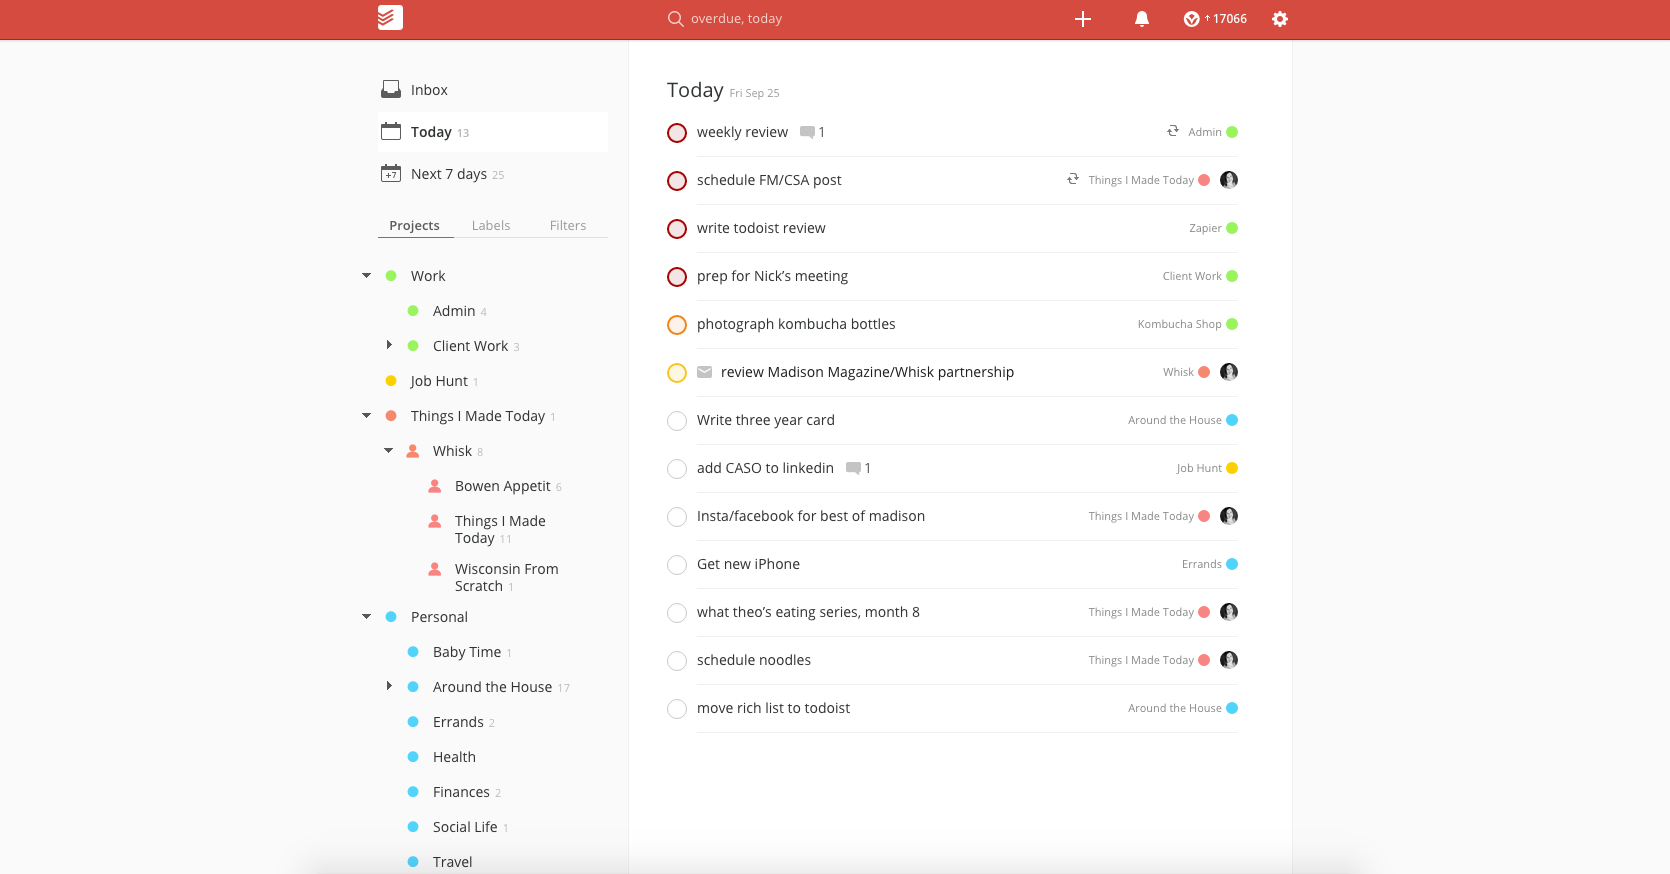
\includegraphics{./tex2pdf.-ae8b3c0afe160db8/224b4a051a5d597717cc2116efe61fed1d4c815d.png}
\caption{Todoist{}}\label{fig:todoist1}
}
\end{figure}

Todoist is the only of these apps which is laser-focused on to-dos. One
of its prominent features is the ability to write tasks in natural
language, which it then understands when they are due, if they are
recurring etc. This is beyond the scope of my product, however I am
interested in the tools they have for tracking your productivity.
Todoist can display graphs of total number of tasks done per day/week,
the distribution between different types of tasks e.g. whether you did
more tasks tagged with ``Study'' or ``Chores''. I definitely want to
have similar visualisations of how productive the user is being.

\begin{figure}
\hypertarget{fig:rtm1}{%
\centering
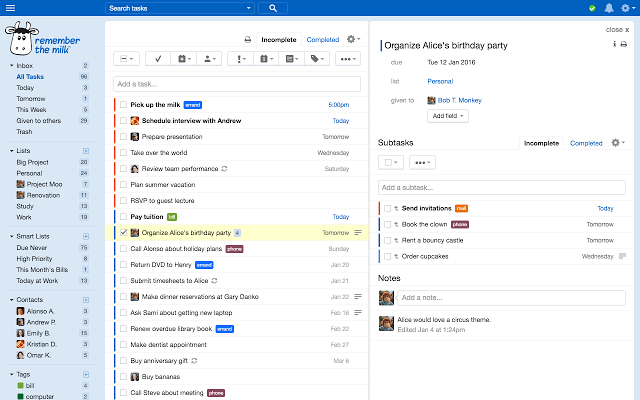
\includegraphics{./tex2pdf.-ae8b3c0afe160db8/243fbf714a614e0b0aee7186756111a073fa79c3.png}
\caption{Remember The Milk{}}\label{fig:rtm1}
}
\end{figure}

Similar to Todoist, Remember the Milk has a lot of advanced tools for
intelligently adding, sorting and searching through tasks. However I'm
particularly interested in the ability to divide tasks into sub-tasks. I
personally have used to-do apps with such a feature and have found it
rather useful, so I'll be interested to get my stakeholder's opinion on
this feature specifically when I talk to them.

\begin{figure}
\hypertarget{fig:ike1}{%
\centering
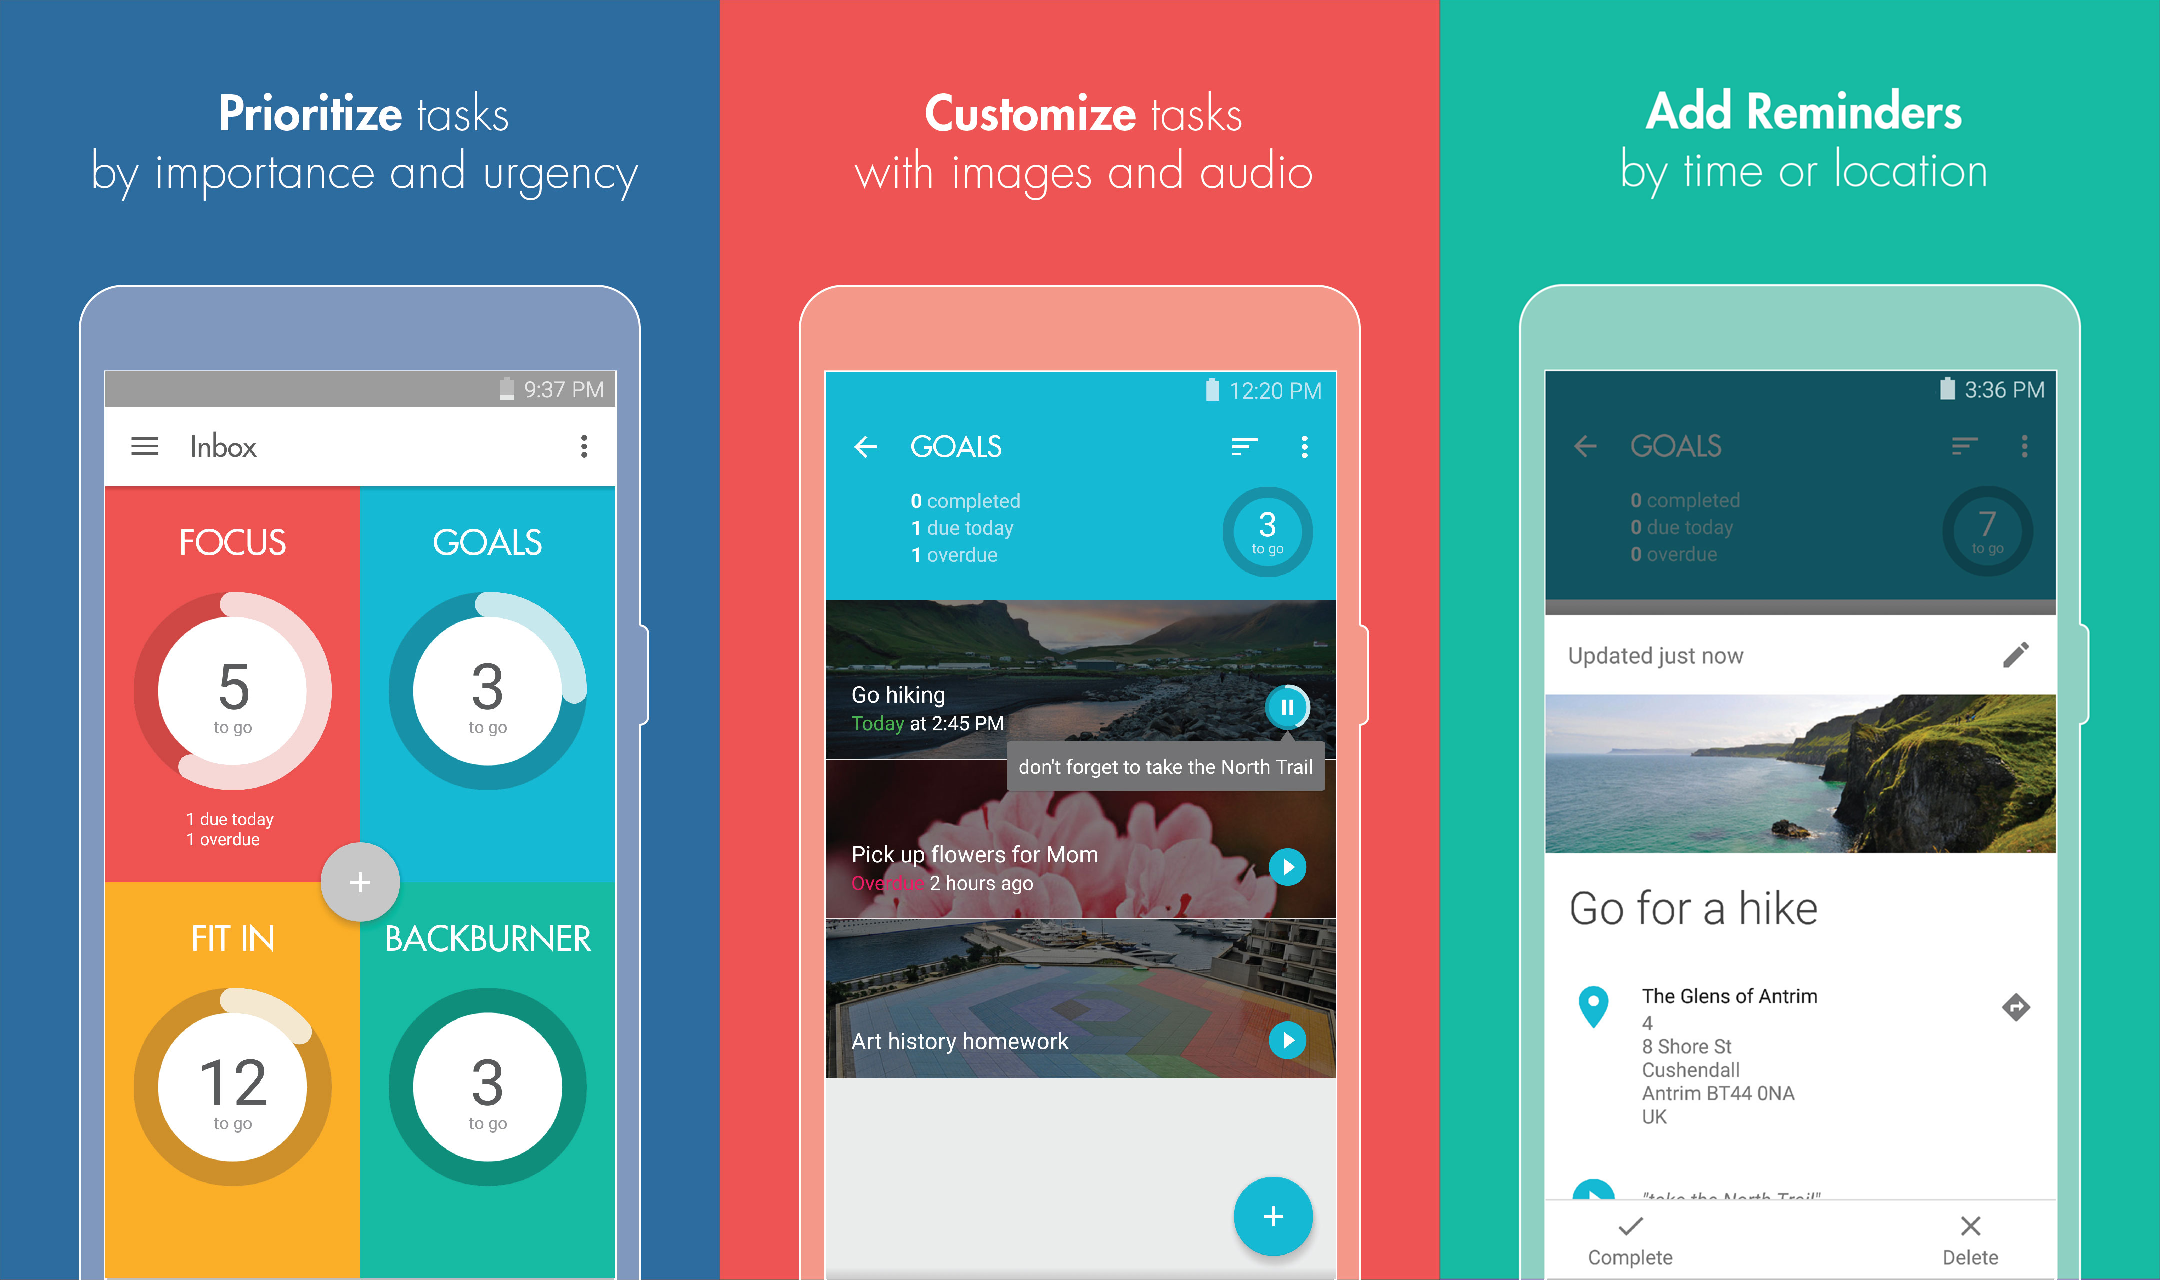
\includegraphics{./tex2pdf.-ae8b3c0afe160db8/514a19219ce1dbefdb0b57c1fa99a8f6e1734dc6.png}
\caption{Ike{}}\label{fig:ike1}
}
\end{figure}

Ike is in fact the to-do app which I currently use. I can't say that I'm
entirely satisfied with it, but I like the system of organising tasks
into ``Urgent and Important'', ``Urgent but not Important'', ``Important
but not Urgent'' and ``Neither Urgent nor Important''. I think this is a
useful system and could perhaps be preset in my product, but I find it
limiting that Ike forces you to organise by those categories. I
definitely want my product to allow the user to organise their tasks
into whatever folders and sub-folders they please. I think any
limitation on how the tasks are organised will always be
counterproductive in some degree to some users.

\begin{figure}
\hypertarget{fig:keep1}{%
\centering
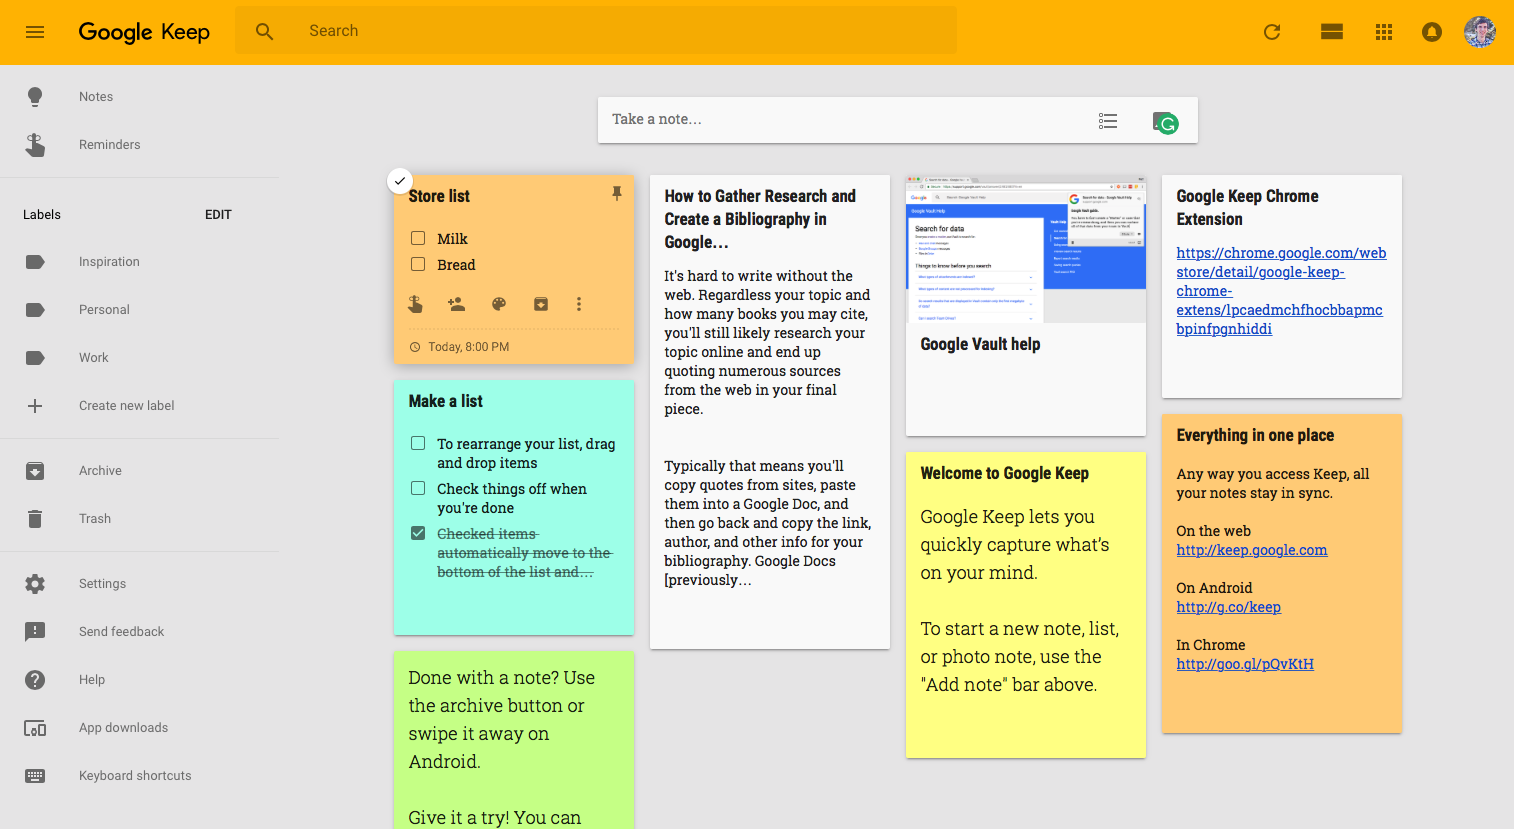
\includegraphics{./tex2pdf.-ae8b3c0afe160db8/fb13cf966f31103aad3d7d246accf11265fada78.png}
\caption{Google Keep{}}\label{fig:keep1}
}
\end{figure}

Keep is quite a good, basic to-do app. Keep's main interesting feature
is its integration with the rest of Google's ecosystem, however this
isn't really something that my project is too concerned with. I'm also
not a fan of Keep's visual metaphor of tasks being ``cards'' on the
screen - a common visual metaphor in Google's design language. I think
this creates confusion as there is not simply a vertical list. I also
dislike that you need to create different types of tasks for simple
text, lists, voice memos etc.

\begin{figure}
\hypertarget{fig:trello1}{%
\centering
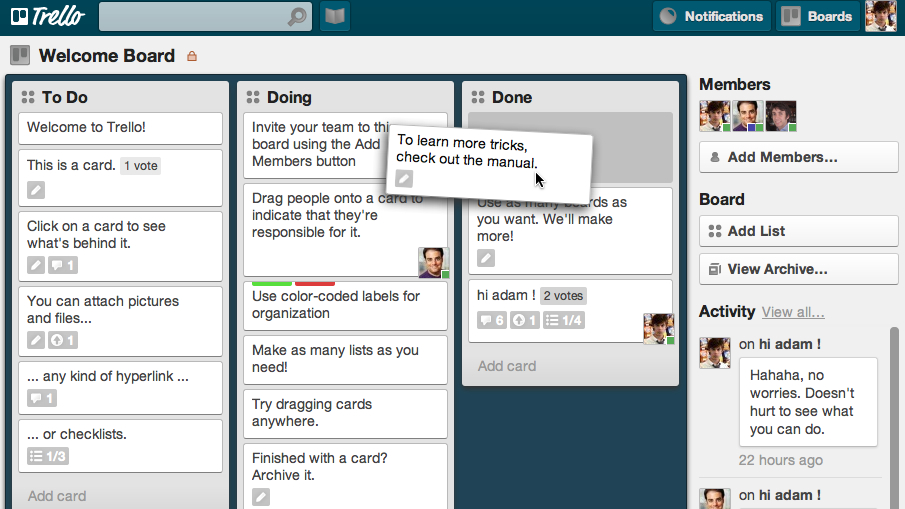
\includegraphics{./tex2pdf.-ae8b3c0afe160db8/a8cbdcbe02b4c5dd114927683b791319dc2cace2.jpg}
\caption{Trello{}}\label{fig:trello1}
}
\end{figure}

Trello is more focused on managing multi-person projects than an
individual's todo list. It's most prominent feature is the ability to
work collaboratively on creating tasks, marking them complete, adding
comments and so on. However I think this sort of feature is beyond the
scope of my solution. However I do like that each ``card'' can - unlike
Keep - have text, checklists, and attachments. I think it will be useful
for my users to be able to attach a reasonable amount of information to
their tasks.

I think these programs all offer partial solutions to the problem, but
none of them offer a solution to the exact problem SH has described.
Forest is excellent for helping you focus on a task, but can't keep
track of your to-dos. Todoist offers excellent functionality for keeping
track of and organising your tasks, but doesn't do anything with regard
to helping you timetable everything that you need to do. Keep is better
in this regard as it integrates with GCal to display tasks in your
calendar, but can't allocate them those time slots automatically. Ike
has a very appealing UI and a good system for organising into four
overarching categories, but you can't create your own categories like
Todoist. Remember the Milk is probably the most intelligent of the
programs, with a ``Smart Add'' feature that makes adding tasks very
simple, and a powerful search for filtering through your tasks, in
addition to integrating with a number of other services such as email
and social media for reminders, and cloud storage services for adding
attachments to tasks, however this is probably beyond the scope of the
problem I'm trying to solve. Evernote is in my opinion the least
effective of these programs, as it is mainly focused on note taking,
with reminders as a side-feature. Trello offers the most features
oriented towards time management and prioritising tasks, but is more
focused around team collaboration on big projects than individual to-do
management.

I showed the candidates to SH to get his opinion and he gave me the
following comments:

Forest: ``This is my favourite. The UI is excellent and the metaphor of
growing trees is very appealing. Out of all the programs this does the
best job of helping me manage my time, however tt's unfortunate that is
doesn't include integrated task management. I like that you can see your
past progress as this is very motivational, and it stops the timer if
you leave the app, which helps you avoid idly switching to Facebook or
Twitter for a 'quick check'.''

Evernote: ``Good for note taking, but that's not really what I'm looking
for. It has too many extraneous features, which are unnecessary and make
it feel bloated - I want a more streamlined experience. I also dislike
the subscription model.''

Todoist: ``Great for managing tasks, with graphs and data to track your
statistics. I love the categorisation and colour coding for different
tasks, and being able to give them different levels of priority. I also
like that you can export your tasks to your calendar. The lack of a dark
mode harms the UX.''

Remember the Milk: ``There's too much task segregation which makes the
UI confusing. It also has a weird notes system. Not a fan.''

Ike: ``The idea behind it is admirable, but ultimately the categories
feel a bit arbitrary, and that's made worse by the lack of an 'all
tasks' view. The UI is very clean however, and the animations are really
nice.''

Keep: ``It's good for lists, but otherwise nothing special.''

Trello: ``Good for project development, but not well-suited to personal
task management.''

He also commented in general that he liked the ability to sync tasks
between devices, and a feature which he wanted but none of the programs
offered was the ability to have ``subtasks'' nestled inside other tasks.

From this I have assembled the following list of features which my
program will need:

\begin{itemize}
\item
  Main view displays all uncompleted tasks and recently completed but
  not-deleted tasks
\item
  Archive containing completed tasks, and allows tasks to be un-marked
  as complete
\item
  Tasks grouped in categories, can be colour coded
\item
  Tasks can be filtered by category
\item
  Ordered by time needed or due date
\item
  Tasks can be marked as done or deleted
\item
  New tasks can be added, with a brief title, optional additional notes,
  an estimate of time needed and a due date
\item
  Graphs showing number of tasks completed, amount of time taken, and
  whether tasks were completed on time
\item
  Show upcoming tasks in their automatically allocated time slots
\item
  User can enter the schedule and other commitments that the program
  will schedule tasks around
\item
  The program will give a warning if there is not enough free time to
  complete a given task before it's due date
\item
  Current task displayed at top of screen
\item
  Time spent working and time to next break
\item
  Buttons to manually pause timer and take a break or mark task as done
\item
  Graphic showing a town/city building up over time as you work
\end{itemize}

I showed this list to SH, and he added that tasks should be given a
priority level, so that high priority tasks can be scheduled before low
priority ones. He also elaborated on the city-building mechanic,
resulting in the following:

\begin{itemize}
\item
  The city builds over time as you work
\item
  Taking a break which has been allocated by the app simply pauses
  development
\item
  Taking an unallocated break sets the development back - perhaps there
  is a level system and you can be set back one or two levels
\item
  If you quit a task before you finished - and taking an excessively
  long break automatically quits - the city is destroyed
\item
  If you take too long to complete a task, development is slowed down
\item
  When you finish a task, you can either stop, which doesn't destroy
  your city but it degrades over time, or go straight to the next task,
  in which case progress continues
\item
  If you finish a task early and go straight on to another task, your
  city gets a boost
\end{itemize}

SH said he ``agrees with all of this'' and called it ``good design''. He
also emphasised his desire to access his tasks across different devices.
I have concluded that the best way to facilitate this would be to build
the program as a web app. This is the easiest way to make it available
cross-platform, as it should be accessible on any device with a modern
web browser.

SH also suggested that there were psychological benefits to offering the
user a choice in what task they do. Studies have shown that individuals
are more motivated to complete a task which they have chosen to do from
a set of options, rather than only one. Therefore I will endeavour to
implement a system which, rather than forcing, or heavily encouraging,
the user to complete one particular task in a certain time slot, will
instead give them the option to choose between tasks with similar levels
of priority.

\hypertarget{system-requirements}{%
\subsubsection{System requirements}\label{system-requirements}}

As the program will be web-based, it will require a system capable of
running a modern internet browser, such as Firefox. The system
requirements for Firefox 66.0 are as follows:

\hypertarget{windows}{%
\paragraph{Windows}\label{windows}}
\addcontentsline{toc}{paragraph}{Windows}

\hypertarget{operating-systems-32-bit-and-64-bit}{%
\subparagraph{Operating Systems (32-bit and
64-bit)}\label{operating-systems-32-bit-and-64-bit}}
\addcontentsline{toc}{subparagraph}{Operating Systems (32-bit and
64-bit)}

\begin{itemize}
\item
  Windows 7
\item
  Windows 8
\item
  Windows 10
\end{itemize}

\hypertarget{recommended-hardware}{%
\subparagraph{Recommended Hardware}\label{recommended-hardware}}
\addcontentsline{toc}{subparagraph}{Recommended Hardware}

\begin{itemize}
\item
  Pentium 4 or newer processor that supports SSE2
\item
  512MB of RAM / 2GB of RAM for the 64-bit version
\item
  200MB of hard drive space
\end{itemize}

\hypertarget{mac}{%
\paragraph{Mac}\label{mac}}
\addcontentsline{toc}{paragraph}{Mac}

\hypertarget{operating-systems}{%
\subparagraph{Operating Systems}\label{operating-systems}}
\addcontentsline{toc}{subparagraph}{Operating Systems}

\begin{itemize}
\item
  macOS 10.9
\item
  macOS 10.10
\item
  macOS 10.11
\item
  macOS 10.12
\item
  macOS 10.13
\item
  macOS 10.14
\end{itemize}

\hypertarget{recommended-hardware_1}{%
\subparagraph{Recommended Hardware}\label{recommended-hardware_1}}
\addcontentsline{toc}{subparagraph}{Recommended Hardware}

\begin{itemize}
\item
  Macintosh computer with an Intel x86 processor
\item
  512 MB of RAM
\item
  200 MB hard drive space
\end{itemize}

\hypertarget{gnulinux}{%
\paragraph{GNU/Linux}\label{gnulinux}}
\addcontentsline{toc}{paragraph}{GNU/Linux}

\hypertarget{software-requirements}{%
\subparagraph{Software Requirements}\label{software-requirements}}
\addcontentsline{toc}{subparagraph}{Software Requirements}

\emph{Please note that GNU/Linux distributors may provide packages for
your distribution which have different requirements.}

\begin{itemize}
\item
  Firefox will not run at all without the following libraries or
  packages:

  \begin{itemize}
  \item
    GTK+ 3.4 or higher
  \item
    GLib 2.22 or higher
  \item
    Pango 1.22 or higher
  \item
    X.Org 1.0 or higher (1.7 or higher is recommended)
  \item
    libstdc++ 4.6.1 or higher
  \end{itemize}
\item
  For optimal functionality, we recommend the following libraries or
  packages:

  \begin{itemize}
  \item
    NetworkManager 0.7 or higher
  \item
    DBus 1.0 or higher
  \item
    GNOME 2.16 or higher
  \item
    PulseAudio
  \end{itemize}
\end{itemize}

Any system which meets these requirements will be able to run the
program.

\hypertarget{success-criteria}{%
\subsubsection{Success Criteria}\label{success-criteria}}

\hypertarget{general-objectives}{%
\paragraph{General objectives}\label{general-objectives}}

To create a program which stores tasks and arranges them around the
user's schedule. The program should engage the user through the use of a
game-like progression system and help the user complete their tasks in a
timely manner through the use of reminders.

\hypertarget{specific-objectives}{%
\paragraph{Specific objectives}\label{specific-objectives}}

The program should:

\begin{itemize}
\item
  Store a list of the user's tasks
\item
  Store the due date, priority, expected time needed, and other
  information about each task
\item
  Add and remove tasks from the list
\item
  Allow the user to group tasks into categories of their choosing, and
  colour code categories
\item
  Record the successful completion of each task, time taken, and number
  of breaks taken and display this information to the user in a useful
  manner
\item
  Schedule time for the user to complete their tasks, according to the
  user's schedule, task due date, task priority, and the user's
  preferences
\item
  Display the tasks in their allocated time slots in a calendar view,
  and allow the user to manually alter time allocations
\item
  Have a focus mode, which helps the user concentrate on the task at
  hand, and incentivise the user to complete the task in a timely manner
  without procrastination using game-like aspects
\item
  Be available on multiple platforms and devices
\item
  Sync tasks between devices
\item
  Remind the user of upcoming tasks
\end{itemize}

\hypertarget{design}{%
\section{Design}\label{design}}

\hypertarget{breaking-down-the-problem}{%
\subsubsection{Breaking down the
problem}\label{breaking-down-the-problem}}

The first step to solving the problem is to decompose it into modules,
which will comprise the overall solution. This is a higher-level
description than the product specification, but low enough that each
component is a manageable individual problem. I have identified the key
functions that my solution will need to perform as:

\begin{itemize}
\item
  Basic calendaring:\\
  My solution needs to keep track of the user's regular commitments, and
  particular events, so that tasks can be scheduled around them.
\item
  Task management:\\
  The user should be able to add tasks, mark them as done, and delete
  them. These tasks should be able to hold a reasonable amount of
  information, but in particular a due date and time estimate will be
  essential to the scheduler.
\item
  Track time spent on tasks:\\
  The user should be able to log they are working on a task, and for how
  long, so that they can see overall statistics, on the accuracy of
  their time estimates, and on how good they are at sticking to their
  schedule.
\item
  Calculate and display statistics:\\
  The aforementioned statistics should be presented to the user in a
  helpful way.
\item
  Scheduling the user's tasks:\\
  The program will need to allocate time for each of the user's tasks,
  according to their priority, due date, and time estimate. It will also
  need to take into account the user's other commitments.
\end{itemize}

\begin{figure}
\hypertarget{fig:TDD1}{%
\centering
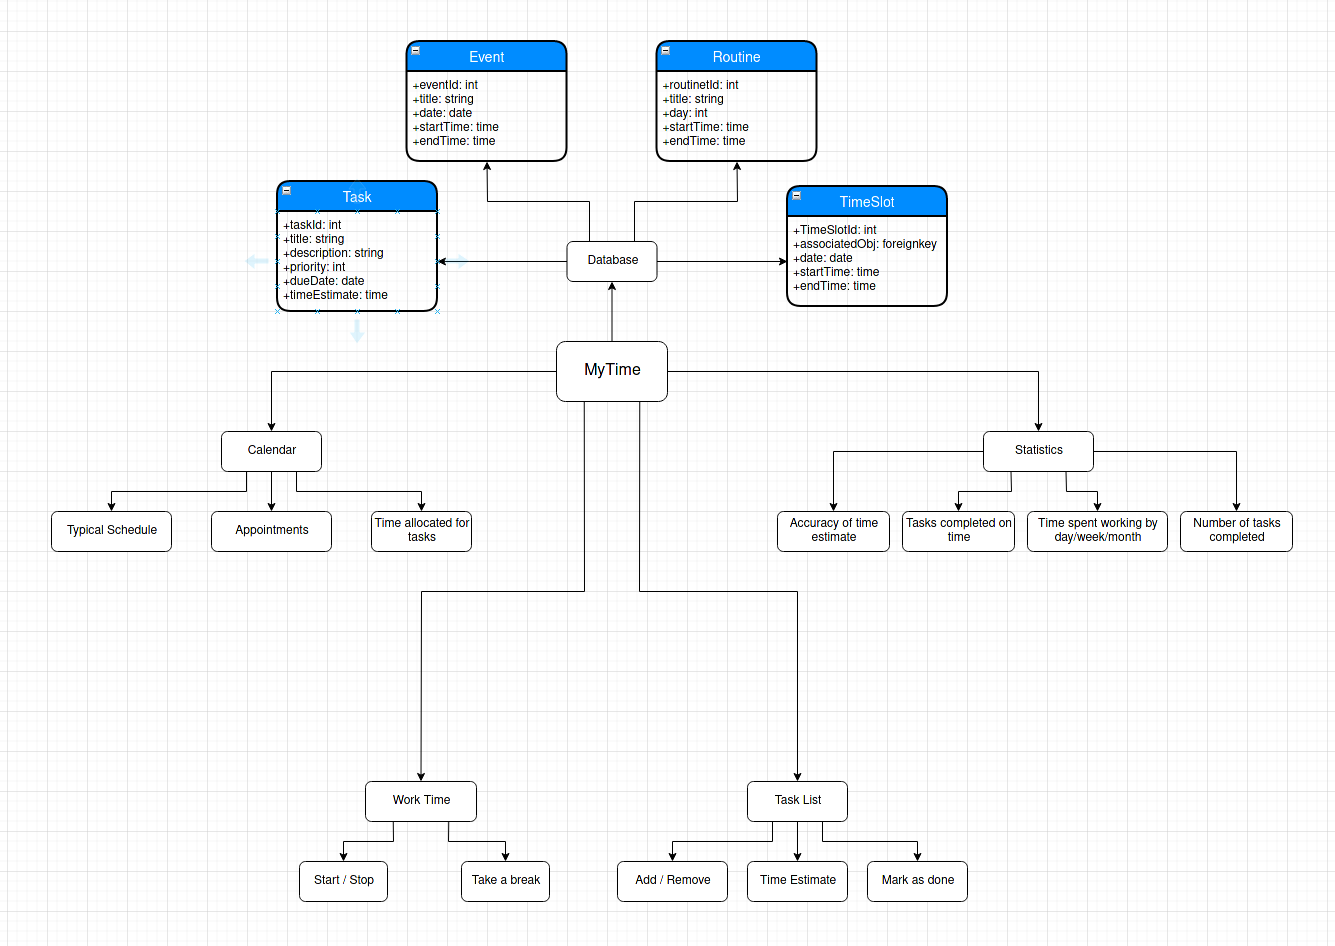
\includegraphics{./tex2pdf.-ae8b3c0afe160db8/7959c99de77473494c0ebd821b4edccdfa48a594.png}
\caption{Combination of top-down design analysis and class
diagrams{}}\label{fig:TDD1}
}
\end{figure}

\hypertarget{explanation-of-design}{%
\subparagraph{Explanation of design}\label{explanation-of-design}}

The solution naturally breaks down into four parts: a task manager, a
basic calendar, a tracker for time spent working, and a statistics
viewer. The relevant data that each component will need to use is also
quite obvious: the task manager, time tracker and statistics tracker
will only be concerned with tasks, whereas the calendar will
additionally need the user's routine, daily commitments, and any
particular events that tasks will need to be scheduled around.

The data, then, will consist of four types. Tasks will have a title and
description, so the user can record a reasonable amount of information
alongside them, and a due date, time estimate and priority level, so
that they can be scheduled. Events and routines are similar, however
differ in that whereas events have a concrete date, routines have a
weekday on which they reoccur. Both have a title, start and end time.
The TimeSlot exists for the purposes of unifying data into a single type
for the purposes of scheduling. They have a data, start and end time as
expected, and additionally an associated object, being the task, event
or routine which occupies that slice of time. It might be possible to
remove the need for this additional data structure, by instead
converting tasks and routines into events for the purpose of scheduling,
however it makes sense to logically distinguish between tasks, events
and routines, which represent user intentions - what the user wants to
do with their time - and time slots, which represent a concrete
allocation of time to be used for a specific purpose. Of course events
and routines are already concrete, as the program will never override
them since this would not be helpful for the user, but it is a nice
logical separation to make in the database, which wouldn't be possible
if I instead used the approach of converting everything into events for
scheduling. Furthermore it would bloat event records with fields that
would often go unused, depending on whether it was a regular event or a
wrapper around a task or routine, so it seems more elegant to have a
separate class for time slots.

\hypertarget{ui-design}{%
\paragraph{UI Design}\label{ui-design}}

It seems sensible for this sort of product that I would want a
navigation bar, shared by every screen, with the content below.

I will have the following views:

\begin{itemize}
\item
  Task list:\\
  A screen where the user can create, view and manage their tasks
\item
  Calendar:\\
  A screen where the user can create, view and manage upcoming events
\item
  Schedule:\\
  A screen showing the users tasks scheduled in around their events for
  today
\item
  Task/event/routine detail:\\
  A screen where the user can look at and individual task, event or
  routine, and perform relevant actions such as marking as done/todo,
  editing or deleting them
\item
  Task/event/routine creator:\\
  A form to create new tasks, events or routines
\item
  Task/event/routine editor:\\
  A form to edit existing tasks, events or routines
\item
  Work time:\\
  A screen where the user can enter a ``work session'' which records the
  time they spend working
\item
  Work review:\\
  A screen displaying statistics about the time the user has spent
  working
\end{itemize}

I think it will be simplest and most intuitive to have a navigation bar,
at the top of the screen, allowing the user to quickly jump between the
five main views - task list, calendar, schedule, work time and work
review - and have individual tasks and events accessible from those
views. It might also be helpful to have a quick button to add a new
task/event/routine.

\hypertarget{development}{%
\section{Development}\label{development}}

\hypertarget{stage-0-learning-django}{%
\subsubsection{Stage 0: Learning Django}\label{stage-0-learning-django}}

I haven't used Django before, so before I really get started on building
my project I need to learn the basics. Fortunately, Django have a very
helpful and comprehensive tutorial, as well as detailed and easy to
navigate documentation.

I decided first of all to run through the standard tutorial, which
involves building a website for hosting various polls. In fact, this
turned out to be incredibly useful because the structure of this website
bears a number of similarities to my project: the main screen is a list
of various polls, which you can then click on to view more information
about and interact with. I will similarly need to have screens with
lists of tasks and events, which you can then view in more detail and
edit or mark as done etc.

\hypertarget{models-and-views}{%
\paragraph{Models and Views}\label{models-and-views}}

I understand that Django is oriented around two primary data structures:
models and views. Models are classes in Python, but they are also the
tables in the database, with the attributes of the class corresponding
to the fields, and instances to specific records. Being objects, they
can also have methods. These don't correspond to anything in the
database, but are useful for manipulating data. I imagine, for example,
that I will want my Task model to have a mark as done method when I come
to implement it.

Views, on the other hand, correspond to the frontend. They outline what
data will be viewed on each page, and also vaguely specify the
appearance of the page, although this is controlled more precisely in
HTML ``templates''.

Here is an example model from the polls tutorial:

\begin{Shaded}
\begin{Highlighting}[]
\KeywordTok{class}\NormalTok{ Question(models.Model):}
\NormalTok{    question_text }\OperatorTok{=}\NormalTok{ models.CharField(max_length}\OperatorTok{=}\DecValTok{200}\NormalTok{)}
\NormalTok{    pub_date }\OperatorTok{=}\NormalTok{ models.DateTimeField(}\StringTok{'date published'}\NormalTok{)}

    \KeywordTok{def} \FunctionTok{__str__}\NormalTok{(}\VariableTok{self}\NormalTok{):}
        \ControlFlowTok{return} \VariableTok{self}\NormalTok{.question_text}

    \KeywordTok{def}\NormalTok{ was_published_recently(}\VariableTok{self}\NormalTok{):}
        \ControlFlowTok{return} \VariableTok{self}\NormalTok{.pub_date }\OperatorTok{>=}\NormalTok{ timezone.now() }\OperatorTok{-}\NormalTok{ datetime.timedelta(days}\OperatorTok{=}\DecValTok{1}\NormalTok{)}
\end{Highlighting}
\end{Shaded}

In the database, this corresponds to a table called ``Question'', with
fields ``question\_text'' and ``pub\_date'', holding text and datetimes
respectively.

Here's a screenshot of the that table:

\begin{figure}
\hypertarget{fig:database1}{%
\centering
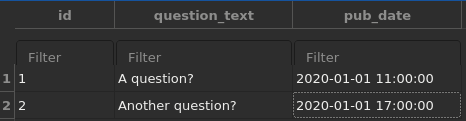
\includegraphics{./tex2pdf.-ae8b3c0afe160db8/d7e757a2f711477f461b1e6dc054f607adf6010c.png}
\caption{Database table ``Question''{}}\label{fig:database1}
}
\end{figure}

As you can see, Django also automatically includes a primary key ``id''
field with each table.

The model also has the methods ``\_\_str\_\_'' and
``was\_published\_recently'', which are not seen in the database, but
rather make it quicker and easier to use the data within Python.

Here is an example view from the polls tutorial:

\begin{Shaded}
\begin{Highlighting}[]
\KeywordTok{class}\NormalTok{ IndexView(generic.ListView):}
\NormalTok{    template_name }\OperatorTok{=} \StringTok{'polls/index.html'}
\NormalTok{    context_object_name }\OperatorTok{=} \StringTok{'latest_question_list'}

    \KeywordTok{def}\NormalTok{ get_queryset(}\VariableTok{self}\NormalTok{):}
        \CommentTok{# Return the last five published questions.}
        \ControlFlowTok{return}\NormalTok{ Question.objects.order_by(}\StringTok{'-pub_date'}\NormalTok{)[:}\DecValTok{5}\NormalTok{]}
\end{Highlighting}
\end{Shaded}

The queryset for this view is the five most recently published objects
in the Question table. It then uses the template located at
``templates/polls/index.html'' - the root folder ``templates'' is
implicit. Here is that template:

\begin{Shaded}
\begin{Highlighting}[]
\NormalTok{\{% if latest_question_list %\}}
   \KeywordTok{<ul>}
\NormalTok{       \{% for question in latest_question_list %\}}
       \KeywordTok{<li><a}\OtherTok{ href=}\StringTok{"/polls/\{\{ question.id \}\}/"}\KeywordTok{>}\NormalTok{\{\{ question.question_text \}\}}\KeywordTok{</a></li>}
\NormalTok{       \{% endfor %\}}
   \KeywordTok{</ul>}
\NormalTok{\{% else \textbackslash{}%\}}
   \KeywordTok{<p>}\NormalTok{No polls are available.}\KeywordTok{</p>}
\NormalTok{\{% endif %\}}
\end{Highlighting}
\end{Shaded}

Unless ``latest\_question\_list'' is empty, this will output a list of
the five most recent questions, showing their names and linking to that
question's page. The URLs are defined in the aptly names urls.py.

\hypertarget{stage-1-tasks}{%
\subsubsection{Stage 1: Tasks}\label{stage-1-tasks}}

Given the foundations laid by my work on the tutorial, I think the best
place to start development will be with task management, especially
given that this is the primary important function of my product.

I need to make:

\begin{itemize}
\item
  A task model, to store that data about each task
\item
  A task index, listing todo and done tasks separately, and linking
  through to view each task in more detail
\item
  A task detail view, showing all the information about a given task and
  allowing editing/deletion
\item
  A form for adding and editing tasks
\item
  A task deletion view
\end{itemize}

\hypertarget{task-model}{%
\paragraph{Task Model}\label{task-model}}

Logically, it makes sense to create the model first, as we can't even
begin to think about how we will display a task until we know their
attributes. Since I've already outlines the attributes and methods for
it in my design, creating the model will be quite simple.

\begin{Shaded}
\begin{Highlighting}[]
\KeywordTok{class}\NormalTok{ Task(models.Model):}
\NormalTok{    LOW }\OperatorTok{=} \DecValTok{1}
\NormalTok{    MED }\OperatorTok{=} \DecValTok{2}
\NormalTok{    HIGH }\OperatorTok{=} \DecValTok{3}
\NormalTok{    PRIORITY_LIST }\OperatorTok{=}\NormalTok{ [}
\NormalTok{        (LOW, }\StringTok{"Low"}\NormalTok{),}
\NormalTok{        (MED, }\StringTok{"Normal"}\NormalTok{),}
\NormalTok{        (HIGH, }\StringTok{"High"}\NormalTok{),}
\NormalTok{    ]}
\NormalTok{    title }\OperatorTok{=}\NormalTok{ models.CharField(max_length}\OperatorTok{=}\DecValTok{200}\NormalTok{)}
\NormalTok{    description }\OperatorTok{=}\NormalTok{ models.CharField(max_length}\OperatorTok{=}\DecValTok{1000}\NormalTok{)}
\NormalTok{    due_date }\OperatorTok{=}\NormalTok{ models.DateField(}\StringTok{"due date"}\NormalTok{)}
\NormalTok{    due_time }\OperatorTok{=}\NormalTok{ models.TimeField(}\StringTok{"due time"}\NormalTok{, default}\OperatorTok{=}\StringTok{"00:00"}\NormalTok{)}
\NormalTok{    time_estimate }\OperatorTok{=}\NormalTok{ models.DurationField(}\StringTok{"time estimate"}\NormalTok{)}
\NormalTok{    priority }\OperatorTok{=}\NormalTok{ models.IntegerField(}\StringTok{"priority"}\NormalTok{, choices}\OperatorTok{=}\NormalTok{PRIORITY_LIST, default}\OperatorTok{=}\DecValTok{2}\NormalTok{)}
\NormalTok{    done }\OperatorTok{=}\NormalTok{ models.BooleanField(default}\OperatorTok{=}\VariableTok{False}\NormalTok{)}

    \KeywordTok{def} \FunctionTok{__str__}\NormalTok{(}\VariableTok{self}\NormalTok{):}
        \ControlFlowTok{return} \VariableTok{self}\NormalTok{.title}

    \KeywordTok{def}\NormalTok{ is_overdue(}\VariableTok{self}\NormalTok{):}
        \ControlFlowTok{return} \VariableTok{self}\NormalTok{.due_date }\OperatorTok{<=}\NormalTok{ timezone.now()}

    \KeywordTok{def}\NormalTok{ mark_done(}\VariableTok{self}\NormalTok{):}
        \VariableTok{self}\NormalTok{.done }\OperatorTok{=} \VariableTok{True}

    \KeywordTok{def}\NormalTok{ mark_todo(}\VariableTok{self}\NormalTok{):}
        \VariableTok{self}\NormalTok{.done }\OperatorTok{=} \VariableTok{False}

    \KeywordTok{def}\NormalTok{ get_absolute_url(}\VariableTok{self}\NormalTok{):}
        \ControlFlowTok{return} \SpecialStringTok{f"/task/}\SpecialCharTok{\{}\VariableTok{self}\SpecialCharTok{.}\BuiltInTok{id}\SpecialCharTok{\}}\SpecialStringTok{/"}
\end{Highlighting}
\end{Shaded}

\end{document}
